\documentclass[a4paper]{article}
\usepackage{amsfonts}
\usepackage{amsmath}
\usepackage{amssymb}
\usepackage{graphicx}
\usepackage{extarrows}

\newcommand{\integral}{\displaystyle\int}
\newcommand{\limit}{\lim\limits}

\begin{document}

\noindent \large Auteur: Seda Jusjajeva\\
\noindent \large Studierichting: Informatica\\
\noindent \large Oefeningenreeks 5K nr. 1.1\\

\medskip

\normalsize


$r = 2\cos\theta$ \\

\begin{figure}[h]
    \centering
    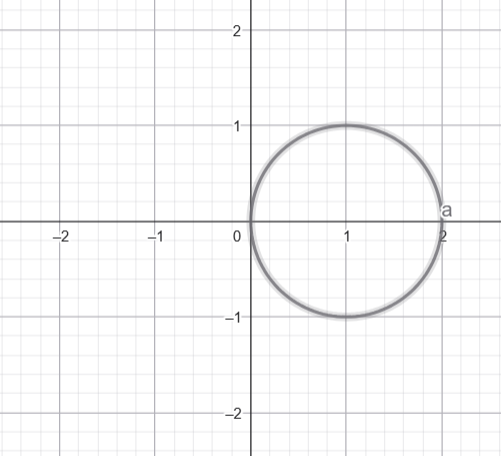
\includegraphics[width=8cm]{5K-1.1-seda.jusjajeva.INF.png}
\end{figure}

$L = 2\integral_0^{\tfrac{\pi}{2}}\sqrt{(2\cos\theta)^2 + ((2\cos\theta)')^2}d\theta$ \\

$\integral\sqrt{(2\cos\theta)^2 + ((2\cos\theta)')^2}d\theta$ \\

$= \integral\sqrt{4\cos^2\theta + 4\sin^2\theta}d\theta$ \\

$= 2\integral\sqrt{1}d\theta$ \\

$= 2\theta + c$ \\

$\Rightarrow L = 2 \left[2\theta\right]_0^{\tfrac{\pi}{2}} = 2\pi$



\begin{thebibliography}{999}
%\bibitem{a} Referentie
\end{thebibliography}
\end{document}